\documentclass[11pt]{beamer}

\usetheme{Boadilla}
\usecolortheme{seahorse}
\usepackage{comment}
\usepackage[utf8]{inputenc}
\usepackage{amsmath,amssymb}
\usepackage{booktabs}
\usepackage{tikz}
\usetikzlibrary{matrix,positioning}

\title[Shared+Private GP]{Multitask Graph GP}

\author[I. Ben Hamza]{In\`es Ben Hamza}

\date[\today]{\today}

\begin{document}

\begin{frame}
\titlepage
\end{frame}



%==================================================

\begin{frame}{Recap: the problem}
\begin{itemize}
    \item \textbf{Setting.} OD calibration = find demand $x$ minimizing
    the gap between simulated and observed link flows. We use Bayesian Optimization with a GP
    surrogate to minimize simulator calls.
    \item \textbf{Multi-output model.} A single simulation returns $L$
    correlated edge flows at once, not one scalar. We model per-edge
    \emph{normalized residuals}
    \[
        r_\ell(x) = \frac{\hat{y}_\ell(x) - y_\ell}{\bar{y}},
        \qquad \bar{y} = \frac{1}{L}\sum_{\ell=1}^L y_\ell,
        \qquad \ell = 1,\dots,L,
    \]
    where $\hat{y}_\ell(x)$ is the simulated flow on edge $\ell$,
    $y_\ell$ the observed ground-truth flow, and $\bar{y}$ the mean
    observed flow across all edges. We then optimize
    \[
        S(x) = C \sum_{\ell=1}^L r_\ell(x)^2 = \text{nRMSE}^2(x),
        \qquad
        C = \frac{L}{\left(\sum_{\ell=1}^L y_\ell\right)^2}.
    \]
\end{itemize}
\end{frame}

\begin{frame}{Research question}
    \begin{itemize}
        \item \textbf{Research question.} Edges sharing routes/junctions are
    physically coupled but does explicitly encoding this via a
    multi-output GP (graph-structured kernel or ICM) improve sample
    efficiency over just fitting an independent GP per edge (IndGP)?
    \item \textbf{Finding.} Across every network tested,
    \textbf{IndGP matched or beat every multi-output variant} so
    inter-edge correlation didn't pay off in practice.
    \end{itemize}

\end{frame}
%==================================================
\begin{frame}{Why the old graph kernel struggles}
Product-kernel graph GP:
\[
    k\bigl((x,\ell),(x',m)\bigr) = k_x(x,x')\,k_{\mathrm{task}}(\ell,m)
\]
\begin{itemize}
    \item Only \textbf{one} input kernel $k_x$, one lengthscale, for
    \emph{every} edge. 
    \item MLL must fit one compromise lengthscale that explains all $L$
    edges' residuals jointly.
    \item If the route-overlap prior misdescribes one edge, that edge has
    \textbf{no private parameters} to fall back on so it's stuck with
    whatever lengthscale best fits everyone else. This is a structural rigidity in the kernel. 
\end{itemize}

\end{frame}

%==================================================
\begin{frame}{Design goal}
Rather than searching for the single best kernel to encode route overlap:
\begin{center}
\Large
\emph{Can we build a kernel \textbf{guaranteed} to do no worse than
IndGP, while still able to exploit route-overlap structure when the data
supports it?}
\end{center}

\end{frame}

%==================================================
\begin{frame}{The new kernel}
\[
    K\bigl((x,\ell),(x',m)\bigr)
    =
    \underbrace{\mathbf{1}[\ell=m]\,\mathrm{priv}_\ell(x,x')}_{\text{per-edge, always present}}
    +
    \underbrace{\rho^2\, k_{\mathrm{shared}}(x,x')\, B_{\ell m}}_{\text{route-overlap correction}}
\]
\begin{itemize}
    \item $\mathrm{priv}_\ell$: independent Mat\'ern-$\tfrac52$ kernel per
    edge $\ell$ so \textbf{own lengthscale, own outputscale}. Identical
    construction to IndGP.
    \item $k_{\mathrm{shared}}$: one Mat\'ern-$\tfrac52$ kernel, one
    lengthscale, shared across all edges. \textbf{No} outputscale
    of its own.
    \item $B \in \mathbb{R}^{L\times L}$: \textbf{fixed} (not learned)
    route-overlap correlation matrix. 
    \item $\rho^2 \geq 0$: single global scalar, learned, representing the strength of
    the shared correction.
    \item Per-edge noise, matching IndGP exactly.
\end{itemize}
\end{frame}

%==================================================
\begin{frame}{Block structure of the kernel}
\begin{center}
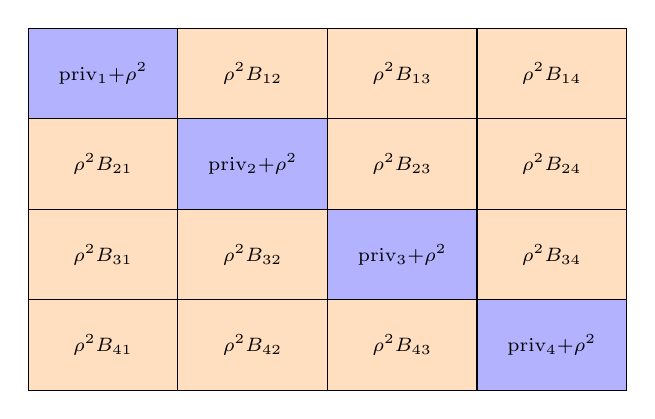
\begin{tikzpicture}[
    cell/.style={draw, minimum width=1.9cm, minimum height=1.15cm,
                 align=center, font=\scriptsize, inner sep=1pt},
    xstep/.style={},
]
    % row 1
    \node[cell, fill=blue!30]   at (0.0,0.0) {priv$_1$+$\rho^2$};
    \node[cell, fill=orange!25] at (1.9,0.0) {$\rho^2 B_{12}$};
    \node[cell, fill=orange!25] at (3.8,0.0) {$\rho^2 B_{13}$};
    \node[cell, fill=orange!25] at (5.7,0.0) {$\rho^2 B_{14}$};
    % row 2
    \node[cell, fill=orange!25] at (0.0,-1.15) {$\rho^2 B_{21}$};
    \node[cell, fill=blue!30]   at (1.9,-1.15) {priv$_2$+$\rho^2$};
    \node[cell, fill=orange!25] at (3.8,-1.15) {$\rho^2 B_{23}$};
    \node[cell, fill=orange!25] at (5.7,-1.15) {$\rho^2 B_{24}$};
    % row 3
    \node[cell, fill=orange!25] at (0.0,-2.3) {$\rho^2 B_{31}$};
    \node[cell, fill=orange!25] at (1.9,-2.3) {$\rho^2 B_{32}$};
    \node[cell, fill=blue!30]   at (3.8,-2.3) {priv$_3$+$\rho^2$};
    \node[cell, fill=orange!25] at (5.7,-2.3) {$\rho^2 B_{34}$};
    % row 4
    \node[cell, fill=orange!25] at (0.0,-3.45) {$\rho^2 B_{41}$};
    \node[cell, fill=orange!25] at (1.9,-3.45) {$\rho^2 B_{42}$};
    \node[cell, fill=orange!25] at (3.8,-3.45) {$\rho^2 B_{43}$};
    \node[cell, fill=blue!30]   at (5.7,-3.45) {priv$_4$+$\rho^2$};
\end{tikzpicture}
\end{center}
\vspace{0.3cm}
\begin{itemize}
    \item \textcolor{blue!60!black}{\textbf{Diagonal (blue)}}: edge $\ell$'s
    own variance, $\mathrm{priv}_\ell(x,x) + \rho^2$ (since
    $k_{\mathrm{shared}}(x,x){=}B_{\ell\ell}{=}1$).
    \item \textcolor{orange!70!black}{\textbf{Off-diagonal (orange)}}: the
    \emph{only} source of cross-edge correlation, entirely from the shared
    term.
    \item $\rho^2 = 0 \Rightarrow$ off-diagonal vanishes $\Rightarrow$
    exactly block-diagonal $\Rightarrow$ exactly IndGP.
\end{itemize}
\end{frame}


%==================================================

\begin{frame}{Full decomposition: all four cases}
The previous slide fixed $x=x'$ (one input, all task pairs). Here is the
general case so same/different edge \emph{and} same/different point:
\footnotesize
\begin{center}
\resizebox{\textwidth}{!}{%
\begin{tabular}{p{3.4cm}ccc}
\toprule
\textbf{Case} & \textbf{Private} & \textbf{Shared} & \textbf{Total $K$} \\
\midrule
Same edge, same pt \newline ($\ell=m,\ x=x'$) &
    $\mathrm{priv}_\ell(x,x)$ &
    $\rho^2$ &
    $\mathrm{priv}_\ell(x,x) + \rho^2$ \\[8pt]
Same edge, diff.\ pt \newline ($\ell=m,\ x\neq x'$) &
    $\mathrm{priv}_\ell(x,x')$ &
    $\rho^2 k_{\mathrm{shared}}(x,x')$ &
    $\mathrm{priv}_\ell(x,x') + \rho^2 k_{\mathrm{shared}}(x,x')$ \\[8pt]
Diff.\ edges, same pt \newline ($\ell\neq m,\ x=x'$) &
    $0$ &
    $\rho^2 B_{\ell m}$ &
    $\rho^2 B_{\ell m}$ \\[8pt]
Diff.\ edges, diff.\ pt \newline ($\ell\neq m,\ x\neq x'$) &
    $0$ &
    $\rho^2 k_{\mathrm{shared}}(x,x') B_{\ell m}$ &
    $\rho^2 k_{\mathrm{shared}}(x,x') B_{\ell m}$ \\
\bottomrule
\end{tabular}%
}
\end{center}
\normalsize
\vspace{0.2cm}
\begin{itemize}
    \item Private term is \textbf{exactly 0} whenever $\ell \neq m$. 
    \item Rows 1 and 3 (the $x=x'$ cases) are exactly the block-structure
    diagram from the previous slide.
    \item Rows 2 and 4 (different points) are what the GP uses to predict
    at new candidate points during BO.
\end{itemize}
\end{frame}

%==================================================
\begin{frame}{Reduction to IndGP as $\rho \to 0$}
\[
    K\bigl((x,\ell),(x',m)\bigr) \;\xrightarrow{\rho^2 \to 0}\;
    \mathbf{1}[\ell=m]\,\mathrm{priv}_\ell(x,x')
\]
\begin{itemize}
    \item Private kernels: same Mat\'ern-$\tfrac52$ family, same
    per-edge lengthscale/outputscale fitting as IndGP.
    \item Noise: per-edge, same as IndGP.

\end{itemize}
\vspace{0.4cm}
\begin{block}{Consequence}
The fitted model can never
be structurally worse than IndGP.
\end{block}
\end{frame}

%==================================================




\begin{frame}{Background reminder: how the usage matrix $M$ is built}
\footnotesize
\textbf{Setup.} $L$ monitored road edges, $D$ OD (origin--destination)
pairs generating demand, $R$ routes total. An OD pair can have several
alternative routes, each chosen with some known probability (the
``split ratio,'' e.g.\ 0.5/0.5 for two equally likely paths).

\vspace{0.1cm}
\textbf{1. Edge--route incidence}, $W \in \{0,1\}^{L\times R}$: \quad
$W_{\ell r} = \mathbf{1}[\text{edge } \ell \text{ lies on route } r]$

\vspace{0.15cm}
\textbf{2. Route--OD split probabilities} (the \texttt{ratio} column in
\texttt{routes.csv}), $W_2 \in [0,1]^{R\times D}$:
\quad $(W_2)_{rd} = \Pr(\text{route } r \mid \text{OD } d)$
\newline \small (each OD pair's routes sum to 1 down that column) \normalsize

\vspace{0.15cm}
\textbf{3. Edge usage}, $M = W W_2 \in [0,1]^{L\times D}$: \quad
$M_{\ell d} = \Pr(\text{edge } \ell \text{ used} \mid \text{OD } d)$

\vspace{0.15cm}
Marginalizes over route choice: the probability a trip for OD pair $d$
passes through edge $\ell$, however it gets routed. 
\end{frame}



%==================================================
\begin{frame}{The $B$ matrix: route-overlap correlation}
\begin{enumerate}
    \item Edge--OD usage matrix $M_{\ell d} = \Pr(\text{edge }\ell\text{ used}\mid \text{OD }d)$
    \item Gram matrix: $G = M M^\top$ \quad (PSD by construction)
    \item Correlation-normalize:
    \[
        B_{\ell m} = \frac{G_{\ell m}}{\sqrt{G_{\ell\ell}\,G_{mm}}}
    \]
\end{enumerate}
\vspace{0.3cm}
\begin{itemize}
    \item $B_{\ell m}$ = cosine similarity between edges $\ell$, $m$'s
    usage vectors (rows of $M$) across all $D$ OD pairs.
    \item Unit diagonal ($B_{\ell\ell}=1$) $\Rightarrow$ gives $\rho^2$ a
    direct variance interpretation:
    \[
        \operatorname{Var}[f_\ell(x)] = \mathrm{priv}_\ell(x,x) + \rho^2
    \]
    \item \textbf{Fixed, not learned} as it is computed once from route data
    before fitting.
\end{itemize}
\end{frame}

%==================================================
\begin{frame}{Fitting challenge: using a prior on $\rho^2$}
\begin{itemize}
    \item Because $B_{\ell\ell}=1$, growing $\rho^2$ inflates every edge's
    variance ``for free'' (private outputscale can just shrink to
    compensate).
    \item Claiming more correlation also looks cheaper to the marginal
    likelihood (smaller determinant), largely regardless of whether it's
    true.
    \item \textbf{Result}: if we let $\rho^2$ go unconstrained, private
    outputscales collapse to $\approx 0$. Hard ceiling alone doesn't fix
    it and $\rho^2$ just pins at whatever ceiling is set (tried 4, 20,
    100).
\end{itemize}
\vspace{0.3cm}
\textbf{Fix}: a soft half-Normal prior on $\rho^2$, added to the MLL
objective. Penalty grows quadratically, so it eventually outweighs the
correlation reward.
On real data: $\rho^2$ settles at $6.13$ (vs.\ pinning at ceiling).
\end{frame}

%==================================================
\begin{frame}{Results: \texttt{grid\_2d\_3x3} ($d=12$, $L=24$, $n_{\mathrm{init}}=5$, 50 iters, 5 seeds)}
\begin{center}
\begin{tabular}{lc}
\toprule
\textbf{Surrogate} & \textbf{Mean best nRMSE} \\
\midrule
ScalarGP & 9.54\% \\
IndGP & 3.18\% \\
GraphGP-Mat\'ern (route-overlap) & 3.18\% \\
\textbf{Shared+Private (new)} & \textbf{2.59\%} \\
\bottomrule
\end{tabular}
\end{center}
\vspace{0.4cm}
\begin{itemize}
    \item $\approx 19\%$ relative improvement over IndGP.
    \item $\approx 19\%$ relative improvement over the old route-overlap
    graph GP.
    \item Lowest variance across seeds of any multi-output surrogate.
\end{itemize}
\end{frame}
%==================================================
\begin{frame}{Convergence: \texttt{grid\_2d\_3x3}}
\begin{figure}
    \centering
    \includegraphics[width=0.82\linewidth]{grid2d_ninit5.png}
    \caption{\tiny Best nRMSE (log scale) vs.\ BO iteration on
    \texttt{grid\_2d\_3x3} ($d=12$ OD pairs, $L=24$ edges, OD bounds
    $[1,1000]^{12}$, $N_0=5$ Sobol init., 50 BO iterations, 5 seeds).
    ScalarGP, IndGP, route-overlap GraphGP-Mat\'ern, Shared+Private
    (Gram $B$), and the \texttt{matern\_spectral} $B$ ablation.}
    \label{fig:grid2d-convergence}
\end{figure}
\end{frame}


%==================================================
\begin{frame}{Results: \texttt{quickstart\_grid\_3} ($d=16$, $L=34$, $n_{\mathrm{init}}=5$, 50 iters, 5 seeds)}
\begin{center}
\begin{tabular}{lc}
\toprule
\textbf{Surrogate} & \textbf{Mean best nRMSE} \\
\midrule
ScalarGP & 8.05\% \\
IndGP & 2.99\% \\
GraphGP-Mat\'ern (route-overlap) & 3.68\% \\
\textbf{Shared+Private (new)} & \textbf{1.52\%} \\
\bottomrule
\end{tabular}
\end{center}
\vspace{0.4cm}
\begin{itemize}
    \item New model beats IndGP on \emph{both} networks. 
\end{itemize}
\end{frame}
%==================================================
\begin{frame}{Convergence: \texttt{quickstart\_grid\_3}}
\begin{figure}
    \centering
    \includegraphics[width=0.82\linewidth]{grid3_ninit5.png}
    \caption{\tiny Best nRMSE (log scale) vs.\ BO iteration on
    \texttt{quickstart\_grid\_3} ($d=16$ OD pairs, $L=34$ edges, OD bounds
    $[1,1000]^{16}$, $N_0=5$ Sobol init., 50 BO iterations, 5 seeds).
    ScalarGP, IndGP, route-overlap GraphGP-Mat\'ern, and the new
    Shared+Private model (Gram $B$).}
    \label{fig:grid3-convergence}
\end{figure}
\end{frame}
%==================================================
\begin{frame}{Ablation: architecture vs.\ $B$-construction (\texttt{grid\_2d\_3x3})}
Isolating \emph{why} the new model wins: additive architecture alone, or
the specific Gram-matrix $B$?
\begin{center}
\begin{tabular}{lc}
\toprule
\textbf{Variant} & \textbf{Mean best nRMSE} \\
\midrule
Route-overlap GraphGP (old, product kernel) & 3.18\% \\
Shared+Private, spectral $B$ (architecture only) & 3.00\% \\
\textbf{Shared+Private, Gram $B$ (full new model)} & \textbf{2.59\%} \\
\bottomrule
\end{tabular}
\end{center}
\vspace{0.4cm}
\begin{itemize}
    \item Additive architecture alone: modest gain ($\approx 6\%$).
    \item Gram-matrix $B$ specifically: the larger contributor.
\end{itemize}
\end{frame}

%==================================================
\begin{comment}{Takeaways}
\begin{itemize}
    \item The old product-kernel graph GPs share one input kernel across
    all edges --- rigid, no private fallback, and this thesis's own
    results show it doesn't reliably beat IndGP.
    \item The new additive shared+private kernel fixes this \textbf{by
    construction}: exact IndGP nesting at $\rho=0$ guarantees it can't be
    structurally worse.
    \item Empirically, it's not just ``no worse'' --- it \textbf{beats}
    IndGP on both networks tested, reversing the thesis's central
    negative result about multi-output surrogates.
    \item Getting $\rho^2$ to fit correctly required recognizing and
    fixing a real MLE degeneracy (soft prior, not just a hard bound).
\end{itemize}
\end{comment}

%==================================================
\begin{comment}{Open questions / next steps}
\begin{itemize}
    \item Run on \texttt{quickstart\_grid\_3\_dense} and additional seeds
    for statistical robustness.
    \item Sensitivity of $\rho^2$'s fitted value to the prior's scale
    $\sigma_\rho$ (currently fixed at 1).
    \item Congestion-scale robustness (0.5$\times$/2$\times$ demand) ---
    partially run, not yet analyzed.
    \item Compare against the pre-existing simpler product-kernel
    ``shared+private'' attempt as an additional baseline.
\end{itemize}
\end{comment}

\end{document}
